\documentclass[
	oneside,
	%openright,
	%titlepage,
	numbers=noenddot,
	%1headlines,
	headinclude,
	footinclude,
	%cleardoublepage=empty,
	abstract=on,
	BCOR=5mm,
	paper=a4,
	fontsize=11pt
]{scrreprt}

\usepackage[utf8]{inputenc}
\usepackage[T1]{fontenc}

\usepackage[
	drafting            = false,       % print version information on the bottom of the pages
	tocaligned          = false,       % the left column of the toc will be aligned (no indentation)
	dottedtoc           = true,        % page numbers in ToC flushed right
	eulerchapternumbers = true,        % use AMS Euler for chapter font (otherwise Palatino)
	linedheaders        = false,       % chaper headers will have line above and beneath
	floatperchapter     = false,       % numbering per chapter for all floats (i.e., Figure 1.1)
	eulermath           = false,       % use awesome Euler fonts for mathematical formulae (only with pdfLaTeX)
	beramono            = true,        % toggle a nice monospaced font (w/ bold)
	palatino            = true,        % deactivate standard font for loading another one, see the last section at the end of this file for suggestions
	style               = arsclassica  % classicthesis, arsclassica
]{classicthesis}

\newcommand{\myTitle}{Generazione sicura di chiavi OpenPGP\xspace}
\newcommand{\mySubtitle}{Guida dettagliata all'uso\xspace}
\newcommand{\myName}{Aldo Latino\xspace}
\newcommand{\myLocation}{Italy\xspace}
\newcommand{\myTime}{1 aprile 2018 -- 14 luglio 2019\xspace}

% \renewcommand{\thefootnote}{\fnsymbol{footnote}}

\usepackage[italian]{babel}

\usepackage{csquotes}

\usepackage[
  %backend=biber,
  bibstyle=alphabetic,%authortitle,
  citestyle=verbose,
  sorting=nty
]{biblatex}
\bibliography{bibliografia}

\usepackage{acronym}

\usepackage{graphicx} %
\usepackage{caption}
\usepackage{subfig}
\graphicspath{{img/}}
%\captionsetup{labelformat=empty} % Rimuove la dicitura "Figura 1" dalle didascalie.
%\captionsetup[subfloat]{labelformat=empty} % Rimuove la numerazione alfabetica delle subfigure.
%\captionsetup{font=scriptsize}
\usepackage{wrapfig}

\usepackage{scrhack} % fix warnings when using KOMA with listings package
\usepackage{xspace} % to get the spacing after macros right

\definecolor{code}{RGB}{233, 30, 99}

\usepackage{tabularx} % better tables
\setlength{\extrarowheight}{3pt} % increase table row height

\usepackage{textcomp}
\usepackage{listings}
%\lstset{emph={trueIndex,root},emphstyle=\color{BlueViolet}}%\underbar} % for special keywords
\lstset{
  language=[LaTeX]Tex,
  morekeywords={PassOptionsToPackage,selectlanguage},
  basicstyle=\small\ttfamily\color{code},
  keywordstyle=\color{RoyalBlue},%\bfseries,
  %identifierstyle=\color{NavyBlue},
  commentstyle=\color{Green}\ttfamily,
  stringstyle=\rmfamily,
  numbers=none,%left,%none
  numberstyle=\scriptsize,%\tiny
  stepnumber=5,
  numbersep=8pt,
  showstringspaces=false,
  breaklines=true,
  %frameround=ftff,
  %frame=single,
  belowcaptionskip=.75\baselineskip,
  upquote=true
  %frame=L
}

\usepackage{classicthesis}

\hypersetup{%
  %draft, % hyperref's draft mode, for printing see below
  colorlinks=true,
  linktocpage=true,
  pdfstartpage=1,
  pdfstartview=FitV,
  % uncomment the following line if you want to have black links (e.g., for printing)
  %colorlinks=false, linktocpage=false, pdfstartpage=3, pdfstartview=FitV, pdfborder={0 0 0},%
  breaklinks=true,
  pageanchor=true,
  pdfpagemode=UseNone,
  % pdfpagemode=UseOutlines,
  plainpages=false,
  bookmarksnumbered,
  bookmarksopen=true,
  bookmarksopenlevel=1,
  hypertexnames=true,
  pdfhighlight=/O,
  % nesting=true,
  % frenchlinks,
  urlcolor=CTurl, linkcolor=CTlink, citecolor=CTcitation, %pagecolor=RoyalBlue,%
  %urlcolor=Black, linkcolor=Black, citecolor=Black, %pagecolor=Black,%
  pdftitle={\myTitle},
  pdfauthor={\myName},
  pdfsubject={\mySubtitle},
  pdfkeywords={Sicurezza, Crittografia, Privacy, GnuPG, OpenPGP},
  pdfcreator={pdfLaTeX},
  pdfproducer={LaTeX with hyperref and ClassicThesis (with ArsClassica)}%
}

\usepackage[italian]{varioref}


\begin{document}

    \frenchspacing

    \title{\myTitle}
    \date{\myTime}

    % Parti di servizio
    \phantomsection
\pdfbookmark[1]{Frontespizio}{frontespizio}

\begin{titlepage}
    \begin{center}
        \hfill

        \vspace{1cm}

        {%
            \fontsize{14pt}{16pt}\selectfont
            \allscsp{\autore}
        }

        \vspace{1cm}

         {%
         \fontsize{18pt}{24pt}\selectfont
         \color{rosso}\addfontfeature{LetterSpace=7}\MakeUppercase{Generazione sicura\\ di chiavi OpenPGP}\par
         }

		\vspace{1cm}

        \emph{\sottotitolo}

        \vspace{1cm}

        \stella

        \vfill

        {%
        \fontsize{10pt}{12pt}\selectfont
        \allscsp{\data}
        }

    \end{center}
\end{titlepage}
    \begingroup
	\footnotesize

	\section*{Sommario}
	Una guida dettagliata, per quanto possibile, sulla generazione,
	conservazione e protezione delle chiavi OpenPGP. La guida è stata pubblicata
	la prima volta su
	\href{https://github.com/aldolat/generazione-sicura-chiavi-openpgp}{GitHub}.

	\section*{Licenza}
	\href{https://creativecommons.org/licenses/by-sa/4.0/deed.it}{
\includegraphics[width=0.09\textwidth]{cc-80x15}
	Creative Commons Attribuzione - Condividi allo stesso modo 4.0 Internazionale
	(CC BY-SA 4.0)} \bigskip

	\noindent La figura \vref{fig:yubikey4} è di proprietà di Yubico.

	\vfill

	\noindent This file was written in \LaTeX~with \textit{ClassicThesis} and
	the \textit{ArsClassica} style.

\endgroup
    \cleardoublepage
\phantomsection

\begingroup
	\pdfbookmark[1]{\contentsname}{tableofcontents}
	\tableofcontents
\endgroup

\cleardoublepage
\phantomsection

\begingroup
    \pdfbookmark[1]{\listtablename}{lot}
	\listoftables
\endgroup


    % Corpo del testo
    \chapter{Introduzione}

Come sappiamo, tutto il sistema della crittografia a chiave
pubblica\footnote{Vedi \cite{wiki:crittografia}.} si basa sull'uso di una chiave
che ha una parte pubblica, da divulgare il più possibile, e una parte privata,
che va tenuta rigorosamente in un luogo sicuro. Qualora avessimo il dubbio che
le chiavi private possano essere in mani altrui, saremmo obbligati a generare un
nuovo mazzo di chiavi, con tutto quello che ne comporta (revoca delle chiavi,
perdita del lavoro fatto per il \emph{Web of
Trust}\footnote{\cite{wiki:webtrust}.}, perdita delle firme apposte sulla nostra
chiave).

Con questa guida vedremo come:

\begin{enumerate}
  \item \emph{generare} in un luogo abbastanza sicuro il nostro mazzo di chiavi
  personale;
  \item \emph{proteggere} le chiavi private in modo da usarle ogni giorno in un
 modo abbastanza sicuro.
\end{enumerate}

Generalmente un mazzo di chiavi personale è composto in modo predefinito da:

\begin{enumerate}
  \item una \emph{chiave master (o principale)} per la firma e la
  certificazione;
  \item una \emph{sottochiave} per la cifratura.
\end{enumerate}

Noi, invece, per elevare la sicurezza del nostro portachiavi spingeremo al
massimo il concetto delle sottochiavi. La struttura del nostro portachiavi
personale, infatti, sarà il seguente:

\begin{itemize}
  \item \emph{Chiave master (o principale) per sola certificazione di chiavi
  altrui} con dimensione 4096 bit e scadenza dopo 3 anni;
  \begin{itemize}
    \item \emph{Sottochiave per firma} con dimensione 2048 bit e scadenza dopo 1
    anno;
    \item \emph{Sottochiave per cifratura} con dimensione 2048 bit e scadenza
    dopo 1 anno;
    \item \emph{Sottochiave per autenticazione} con dimensione 2048 bit e
    scadenza dopo 1 anno.
  \end{itemize}
\end{itemize}

Avremo quindi \emph{una chiave distinta per ogni operazione}.

La chiave più importante è la \emph{chiave master}. Questa chiave è talmente
importante che, qualora fosse stata compromessa, ci costringerebbe a revocare
l'intero mazzo di chiavi e a generarne di nuove. Per questo motivo la terremo in
cassaforte, separata dal resto del mazzo di chiavi. Visto che la terremo
separata dal resto, la abiliteremo solo per scopi che non sono quotidiani, ma
periodici (come ad esempio il rinnovo della validità delle chiavi) o per
occasioni speciali (come ad esempio un \emph{Key signing
party}\footnote{\cite{wiki:ksp}.}). Lo scopo della chiave master sarà quello di
certificare chiavi altrui ed, essendo la chiave principale, di effettuare
operazioni di manutenzione del nostro mazzo di chiavi (estensione validità,
aggiunta di nomi utente, ecc.).

Le \emph{sottochiavi}, invece, saranno utilizzate quotidianamente. Le
sottochiavi hanno la caratteristica che possono esistere nel portachiavi di
GnuPG anche senza la presenza della chiave principale. Per questo motivo, dopo
aver fatto un sicuro backup, elimineremo dal portachiavi la chiave principale,
lasciando solo le sottochiavi. Le sottochiavi, per loro natura, potrebbero anche
essere compromesse (cosa che non dobbiamo permettere mai e, a tal scopo, vedremo
come proteggerle), ma questo non invaliderebbe l'intero mazzo di chiavi: qualora
una sottochiave fosse compromessa, potremmo revocarla e crearne un'altra per lo
stesso scopo. Le sottochiavi potrebbero anche scadere e, qualora non volessimo
rinnovarle, potremmo generarne di nuove. Oppure potremmo generare una
sottochiave per un evento particolare (un convegno o altro), che ha quindi una
durata limitata (un mese, un anno) e lasciarla scadere dopo la fine dell'evento.

\begin{wrapfloat}{figure}{r}{0pt}
    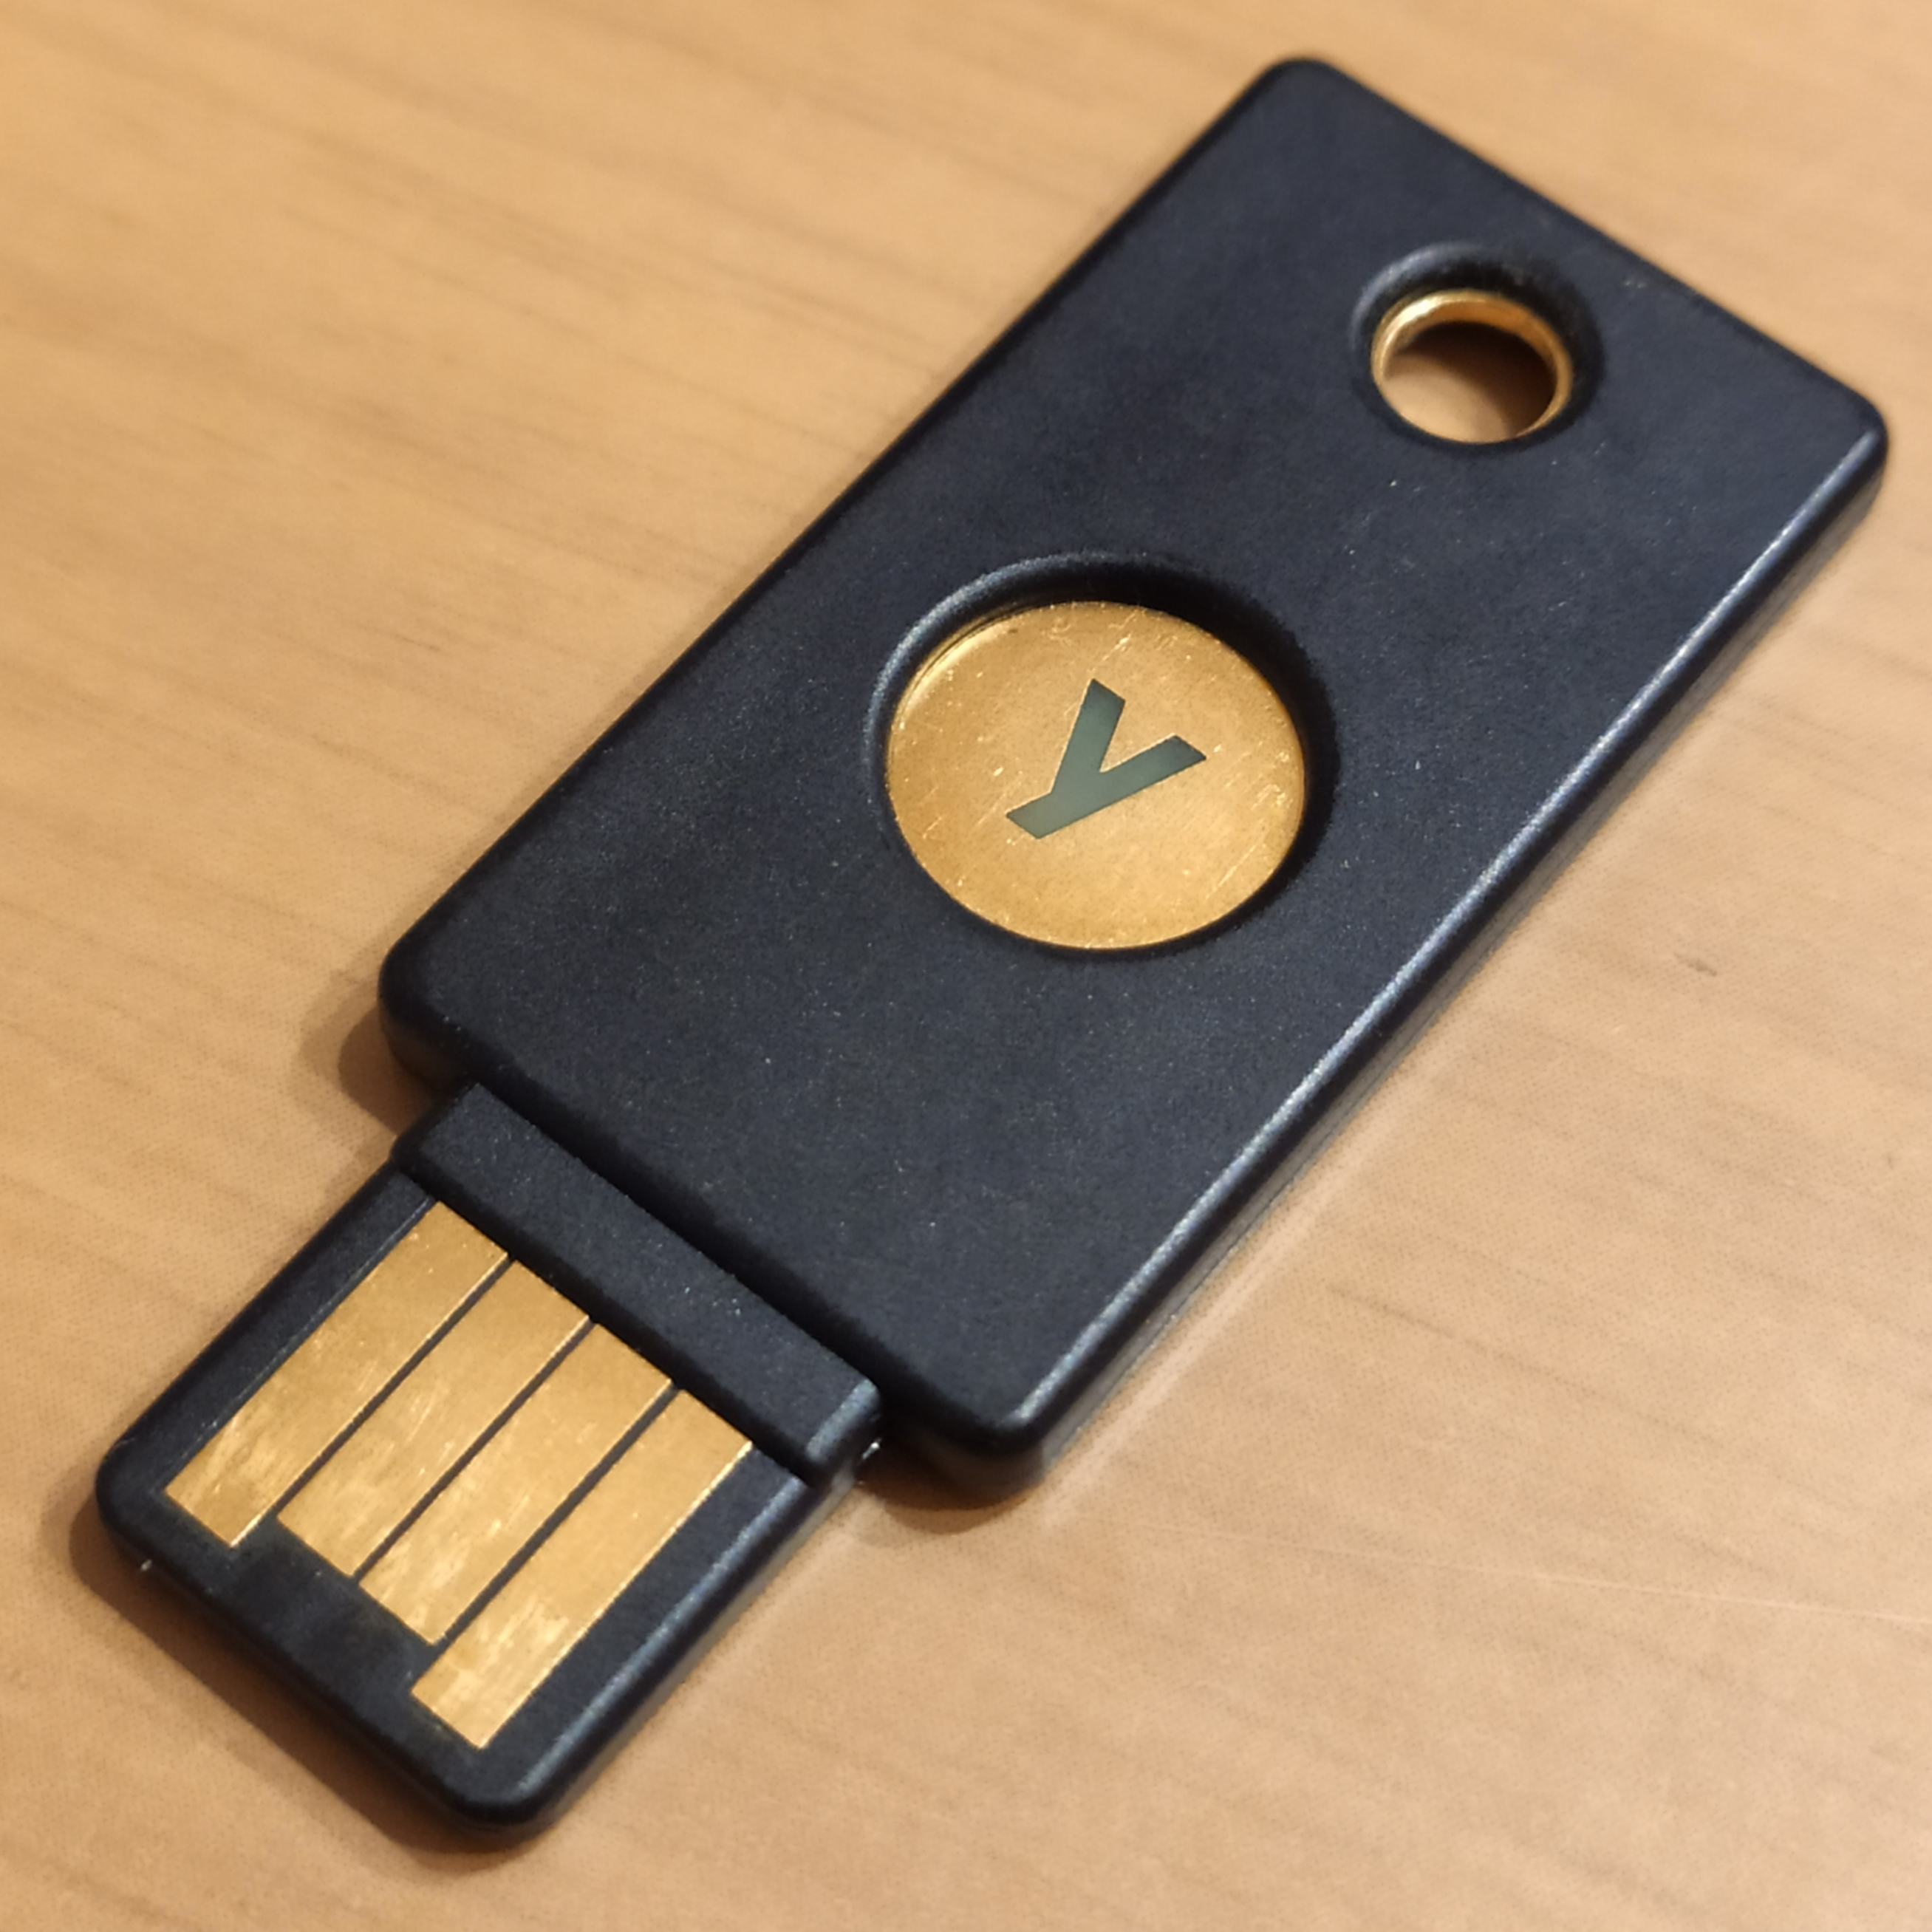
\includegraphics[width=0.33\textwidth]{yubikey4}
    \caption{La YubiKey 4 di Yubico.}
    \label{fig:yubikey4}
\end{wrapfloat}

Per proteggere le nostre sottochiavi, le sposteremo su \emph{un token
\textsc{usb} come la YubiKey}.\footnote{\url{https://www.yubico.com/}.} Si
tratta di token praticamente indistruttibili, che rendono l'uso della firma
digitale, la cifratura e l'autenticazione su sistemi (come \textsc{ssh}) molto
comodi, dato che basterà usare un \textsc{pin} numerico al posto della
passphrase. Io uso la YubiKey
4,\footnote{\url{https://www.yubico.com/product/yubikey-4-series/\#yubikey-4}}
come da figura \ref{fig:yubikey4}. I token come YubiKey hanno il pregio che non
permettono l'esportazione delle chiavi lì conservate; questo significa che posso
usare le mie chiavi anche in un ambiente poco sicuro come un Internet Point, un
\textsc{pc} condiviso, ecc., senza il timore che le chiavi private possano
essere copiate da qualche parte a mia insaputa. Quand'anche fosse stato
intercettato il \textsc{pin} da un keylogger o da un malware, la passphrase è
ancora al sicuro, ed eventualmente posso cambiare il \textsc{pin}. Il fatto che
le sottochiavi, una volta trasferite, non possano essere esportate dalla
YubiKey, ci forzerà a effettuare il backup del nostro mazzo di chiavi prima del
trasferimento, ma questo aspetto lo vedremo al momento opportuno.

Alla fine della guida avremo quindi la seguente situazione:

\begin{enumerate}
  \item \emph{la chiave principale} sarà rimossa dal portachiavi sul disco e trasferita
  in un luogo sicuro;
  \item \emph{le sottochiavi} risiederanno sulla YubiKey.
\end{enumerate}

Nel nostro disco fisso non avremo quindi nessuna chiave privata. Potremmo anche
perdere il nostro \textsc{pc} o potrebbero anche rubarcelo, ma il nostro mazzo
di chiavi sarà sempre al sicuro. Potremmo anche perdere la nostra YubiKey, ma
essa contiene solo le sottochiavi che, come abbiamo visto, possiamo revocare con
la chiave principale (che sta in cassaforte) e ricrearne di nuove. Quando sarà
necessario effettuare un'operazione speciale, come ad esempio apporre la nostra
firma su chiavi altrui o aggiungere/eliminare una sottochiave o una UserID,
importeremo la chiave principale nel nostro portachiavi, effettueremo
l'operazione necessaria e infine la rimuoveremo di nuovo.\bigskip

\noindent Un ultimo punto prima di passare alla pratica. Il motivo di avere una
scadenza sulle chiavi è un ulteriore sicurezza per noi. Immaginiamo il caso in
cui dovessimo perdere il controllo del nostro mazzo di chiavi, compresa la
chiave principale, e non avessimo più a disposizione nemmeno il certificato di
revoca. In questo caso la scadenza sarà una garanzia per noi che a un certo
punto le chiavi scadranno in modo naturale. Per i tempi di scadenza ognuno può
scegliere quello che più ritenga opportuno, ma 3 anni per la principale e 1 anno
per le sottochiavi dovrebbe essere un buon compromesso tra la seccatura di dover
manutenzionare il portachiavi e il tempo di scadenza naturale dopo eventuale
compromissione.\bigskip

\noindent Questa guida può essere seguita in modo modulare:

\begin{itemize}
  \item si può scegliere di mantenere tutte le chiavi sul proprio disco fisso,
  seguendo solo la parte sulla generazione sicura delle chiavi;
  \item si può scegliere di spostare in un luogo sicuro la chiave principale dal
  resto del proprio mazzo di chiavi, mantenendo nel disco fisso solo le
  sottochiavi;
  \item si può scegliere di spostare le sottochiavi in un token \textsc{usb}
  come la YubiKey, mantenendo la chiave principale nel disco fisso;
  \item si può scegliere di spostare le sottochiavi in un token \textsc{usb}
  come la YubiKey e di spostare la chiave principale in un luogo sicuro, non
  lasciando nessuna chiave privata nel disco fisso.
\end{itemize}\bigskip

\noindent Una nota prima di cominciare. Lungo la guida i vari comandi da
terminale useranno \textsc{id} di chiave, keygrip, percorsi nel disco fisso e
quant'altro che fanno riferimento a quanto eseguito per scrivere la guida. Ciò
significa che dovrete sostituire gli \textsc{id} di chiave, i keygrip, i
percorsi e quant'altro con quelli vostri. Ad esempio, in un comando come questo:

\begin{lstlisting}
gpg --with-keygrip --list-key 0x9F676B5A4B6E6777
\end{lstlisting}

\noindent dovrete sostituire \texttt{0x9F676B5A4B6E6777} con l'\textsc{id}
corretto della vostra chiave.

Inoltre, il percorso \texttt{/home/user} va modificato inserendo il nome utente
corretto al posto di \texttt{user}.

    \section{Generazione delle chiavi}

Con questa guida genereremo la nostra chiave privata che avrà questo schema:

\begin{itemize}
    \item \emph{Chiave master (o principale)} [C -- Certification/Certificazione]
    \begin{itemize}
        \item \emph{Sottochiave per firma} [S -- Signing/Firma]
        \item \emph{Sottochiave per cifratura} [E -- Encryption/Cifratura]
        \item \emph{Sottochiave per autenticazione} [A --
    Authentication/Autenticazione]
    \end{itemize}
\end{itemize}

Per la lunghezza delle chiavi avremo la chiave primaria a 4096 bit
mentre le sottochiavi a 2048 bit.\footnote{Per ulteriori informazioni su questo
dibattito della lunghezza delle chiavi si può vedere: \cite{gnupg:keylength} e
anche \cite{yubico:keylength}.}

\subsection{Prerequisiti}

\begin{enumerate}
 \item È necessario lavorare su un sistema avviato con una distribuzione Linux
 in modalità \textit{live}. È preferibile una
 \href{https://tails.boum.org/index.it.html}{Tails}, ma va bene una qualunque.
 La distribuzione va avviata isolandola da qualsiasi rete.
 \item È necessario usare GnuPG versione 2.1 o successiva.
 \item È necessario un token \textsc{usb} come, ad esempio, una YubiKey, nel
 caso si decida di spostare le sottochiavi su questo supporto.
\end{enumerate}

Qualora il comando \texttt{gpg} lanci GnuPG versione 1, accertarsi che
la versione 2 sia installata e aggiungere questa riga al seguente file:
\texttt{/home/user/.bash\_aliases}:

\begin{lstlisting}
alias gpg='gpg2'
\end{lstlisting}

Questa scorciatoia permetterà l'avvio di GnuPG versione 2 ogni volta
che digitiamo \texttt{gpg}.

\subsection{Generare le chiavi}

Sul sistema di generazione delle chiavi accertarsi di avere GnuPG versione 2.1 o
successiva:

\begin{lstlisting}
gpg --version
\end{lstlisting}

Iniziare quindi la procedura con:

\begin{lstlisting}
gpg --expert --full-gen-key
\end{lstlisting}

che darà:

\begin{lstlisting}
Please select what kind of key you want:
   (1) RSA and RSA (default)
   (2) DSA and Elgamal
   (3) DSA (sign only)
   (4) RSA (sign only)
   (7) DSA (set your own capabilities)
   (8) RSA (set your own capabilities)
   (9) ECC and ECC
  (10) ECC (sign only)
  (11) ECC (set your own capabilities)
Your selection?
\end{lstlisting}

Scegliamo \texttt{8}:

\begin{lstlisting}
Possible actions for a RSA key: Sign Certify Encrypt Authenticate
Current allowed actions: Sign Certify Encrypt

   (S) Toggle the sign capability
   (E) Toggle the encrypt capability
   (A) Toggle the authenticate capability
   (Q) Finished

Your selection?
\end{lstlisting}

Come si vede le attuali capacità della chiave che stiamo creando sono:
\texttt{Sign Certify Encrypt}. Rimuoviamo le capacità di firma premendo
\texttt{S}:

\begin{lstlisting}
Possible actions for a RSA key: Sign Certify Encrypt Authenticate
Current allowed actions: Certify Encrypt

   (S) Toggle the sign capability
   (E) Toggle the encrypt capability
   (A) Toggle the authenticate capability
   (Q) Finished

Your selection?
\end{lstlisting}

Rimuoviamo le capacità di cifratura premendo \texttt{E}:

\begin{lstlisting}
Possible actions for a RSA key: Sign Certify Encrypt Authenticate
Current allowed actions: Certify

   (S) Toggle the sign capability
   (E) Toggle the encrypt capability
   (A) Toggle the authenticate capability
   (Q) Finished

Your selection?
\end{lstlisting}

Ora la chiave primaria avrà solo la capacità di certificazione
(\texttt{Certify}) su altre chiavi.

Premiamo \texttt{Q}:

\begin{lstlisting}
RSA keys may be between 1024 and 4096 bits long.
What keysize do you want? (2048)
\end{lstlisting}


Inserire \texttt{4096}:

\begin{lstlisting}
Requested keysize is 4096 bits
Please specify how long the key should be valid.
         0 = key does not expire
      <n>  = key expires in n days
      <n>w = key expires in n weeks
      <n>m = key expires in n months
      <n>y = key expires in n years
Key is valid for? (0)
\end{lstlisting}


Inseriamo \texttt{3y} (3 anni):

\begin{lstlisting}
Key expires at mer 31 mar 2021 19:46:05 CEST
Is this correct? (y/N)
\end{lstlisting}

Premiamo \texttt{Y}:

\begin{lstlisting}
GnuPG needs to construct a user ID to identify your key.

Real name:
Email address:
Comment:
\end{lstlisting}


Inseriamo il nostro nome e cognome e quindi l'indirizzo email. Come commento
lasciamo il campo vuoto.

\begin{lstlisting}
You selected this USER-ID:
    "Mario Rossi <mario.rossi@example.com>"

Change (N)ame, (C)omment, (E)mail or (O)kay/(Q)uit?
\end{lstlisting}

Accettare con \texttt{O}:

\begin{lstlisting}
We need to generate a lot of random bytes. It is a good idea to perform
some other action (type on the keyboard, move the mouse, utilize the
disks) during the prime generation; this gives the random number
generator a better chance to gain enough entropy.
\end{lstlisting}

A seguire GnuPG chiederà di impostare la passphrase.

Impostiamo la passphrase.

\begin{lstlisting}
gpg: key 4B6E6777 marked as ultimately trusted
gpg: directory '/home/mariorossi/.gnupg/openpgp-revocs.d' created
gpg: revocation certificate stored as '/home/mariorossi/.gnupg/openpgp-revocs.d/491532759708014725CFE3A79F676B5A4B6E6777.rev'
public and secret key created and signed.

gpg: checking the trustdb
gpg: marginals needed: 3  completes needed: 1  trust model: PGP
gpg: depth: 0  valid:   1  signed:   0  trust: 0-, 0q, 0n, 0m, 0f, 1u
gpg: next trustdb check due at 2021-03-31
pub   rsa4096/4B6E6777 2018-04-01 [C] [expires: 2021-03-31]
      Key fingerprint = 4915 3275 9708 0147 25CF  E3A7 9F67 6B5A 4B6E 6777
uid         [ultimate] Mario Rossi <mario.rossi@example.com>
\end{lstlisting}

GnuPG mostra la chiave appena generata ed esce.

Come si vede, esiste solo la chiave principale con la sola capacità di
certificazione \texttt{[C]}. Bisogna ora generare le sottochiavi con:

\begin{lstlisting}
gpg --expert --edit-key 0x4B6E6777
\end{lstlisting}


\begin{lstlisting}
gpg (GnuPG) 2.1.11; Copyright (C) 2016 Free Software Foundation, Inc.
This is free software: you are free to change and redistribute it.
There is NO WARRANTY, to the extent permitted by law.

Secret key is available.

sec  rsa4096/4B6E6777
     created: 2018-04-01  expires: 2021-03-31  usage: C
     trust: ultimate      validity: ultimate
[ultimate] (1). Mario Rossi <mario.rossi@example.com>

gpg>
\end{lstlisting}

Dare il comando \texttt{addkey}:

\begin{lstlisting}
Please select what kind of key you want:
   (3) DSA (sign only)
   (4) RSA (sign only)
   (5) Elgamal (encrypt only)
   (6) RSA (encrypt only)
   (7) DSA (set your own capabilities)
   (8) RSA (set your own capabilities)
  (10) ECC (sign only)
  (11) ECC (set your own capabilities)
  (12) ECC (encrypt only)
  (13) Existing key
Your selection?
\end{lstlisting}

Scegliere \texttt{8}:

\begin{lstlisting}
Possible actions for a RSA key: Sign Encrypt Authenticate
Current allowed actions: Sign Encrypt

   (S) Toggle the sign capability
   (E) Toggle the encrypt capability
   (A) Toggle the authenticate capability
   (Q) Finished

Your selection?
\end{lstlisting}

Togliere la capacità di cifratura premendo \texttt{E}:

\begin{lstlisting}
Possible actions for a RSA key: Sign Encrypt Authenticate
Current allowed actions: Sign

   (S) Toggle the sign capability
   (E) Toggle the encrypt capability
   (A) Toggle the authenticate capability
   (Q) Finished

Your selection?
\end{lstlisting}

Scegliere \texttt{Q}:

\begin{lstlisting}
RSA keys may be between 1024 and 4096 bits long.
What keysize do you want? (2048)
\end{lstlisting}

Premere \texttt{Invio} per accettare \texttt{2048}:

\begin{lstlisting}
Requested keysize is 2048 bits
Please specify how long the key should be valid.
         0 = key does not expire
      <n>  = key expires in n days
      <n>w = key expires in n weeks
      <n>m = key expires in n months
      <n>y = key expires in n years
Key is valid for? (0)
\end{lstlisting}

Inserire \texttt{1y} per farla scadere dopo 1 anno:

\begin{lstlisting}
Key expires at lun 01 apr 2019 19:57:16 CEST
Is this correct? (y/N)
\end{lstlisting}

Accettare inserendo \texttt{Y}:

\begin{lstlisting}
Really create? (y/N)
\end{lstlisting}

Accettare inserendo \texttt{Y}.

Inserire quindi la passphrase e la sottochiave sarà aggiunta al portachiavi:

\begin{lstlisting}
We need to generate a lot of random bytes. It is a good idea to perform
some other action (type on the keyboard, move the mouse, utilize the
disks) during the prime generation; this gives the random number
generator a better chance to gain enough entropy.
\end{lstlisting}


Attendiamo che finisca, quindi apparirà:

\begin{lstlisting}
sec  rsa4096/4B6E6777
     created: 2018-04-01  expires: 2021-03-31  usage: C
     trust: ultimate      validity: ultimate
ssb  rsa2048/9114F367
     created: 2018-04-01  expires: 2019-04-01  usage: S
[ultimate] (1). Mario Rossi <mario.rossi@example.com>

gpg>
\end{lstlisting}


Aggiungiamo ora con la stessa procedura (partendo da \texttt{addkey}) la chiave
di cifratura e poi quella di autenticazione. Alla fine, dopo aver aggiunto la
sottochiave di autenticazione, dare il comando:

\begin{lstlisting}
save
\end{lstlisting}

per salvare e uscire.

Alla fine avremo questo portachiavi:

\begin{lstlisting}
gpg --list-secret-keys
\end{lstlisting}


\begin{lstlisting}
/home/mariorossi/.gnupg/pubring.kbx
-----------------------------
sec   rsa4096/4B6E6777 2018-04-01 [C] [expires: 2021-03-31]
uid         [ultimate] Mario Rossi <mario.rossi@example.com>
ssb   rsa2048/9114F367 2018-04-01 [S] [expires: 2019-04-01]
ssb   rsa2048/2F3AC08A 2018-04-01 [E] [expires: 2019-04-01]
ssb   rsa2048/AFBE0F10 2018-04-01 [A] [expires: 2019-04-01]
\end{lstlisting}

La situazione è, quindi, la seguente:

\begin{itemize}
    \item \emph{chiave principale}, adibita alla sola \emph{certificazione e
    gestione del portachiavi}: \newline \texttt{sec   rsa4096/4B6E6777 2018-04-01
    [C]};
    \item \emph{sottochiave di firma}: \newline \texttt{ssb   rsa2048/9114F367
    2018-04-01 [S]};
    \item \emph{sottochiave di cifratura}: \newline \texttt{ssb
    rsa2048/2F3AC08A 2018-04-01 [E] [expires: 2019-04-01]};
    \item \emph{sottochiave di autenticazione}: \newline \texttt{ssb
    rsa2048/AFBE0F10 2018-04-01 [A] [expires: 2019-04-01]}.
\end{itemize}

Possiamo aggiungere anche altri UserID o una foto con:

\begin{lstlisting}
gpg --expert --edit-key 0x4B6E6777
\end{lstlisting}

e poi con \texttt{adduid}.

\subsection{Il certificato di revoca}
\label{certificato-revoca}

Con GnuPG versione 2 la generazione del certificato di revoca è stata fatta
automaticamente quando le chiavi sono state generate e si trova nella
directory \texttt{/home/user/.gnupg/openpgp-revocs.d/}. Il file ha lo
stesso nome dell'impronta della chiave, nel nostro caso:

\begin{lstlisting}
491532759708014725CFE3A79F676B5A4B6E6777.rev
\end{lstlisting}

Questo file andrà tolto da questa directory e conservato in un luogo sicuro. Lo
vedremo nel paragrafo \vref{backup-certificato-revoca} dedicato al backup.

\subsection{Impostare le preferenze della chiave}

Modificare la chiave con:

\begin{lstlisting}
gpg --expert --edit-key 0x4B6E6777
\end{lstlisting}

Dal prompt di Gnupg dare:

\begin{lstlisting}
setpref S10 S9 S8 H10 H9 H8 Z2 Z3 Z1 Z0
\end{lstlisting}

Per il significato dei codici, vedi la Tabella \vref{table:codici}.

\begin{table}
   \centering
	\begin{tabularx}{6cm}{cl}
 		\toprule
		\textsc{Codice} & \textsc{Descrizione} \\
		\midrule
		\texttt{S10} & Cifrario Twofish \\
		\texttt{S9}  & Cifrario \numerimaiuscoli{AES256} \\
		\texttt{S8}  & Cifrario \numerimaiuscoli{AES192} \\
		\texttt{H10} & Hash \numerimaiuscoli{SHA512} \\
		\texttt{H9}  & Hash \numerimaiuscoli{SHA384} \\
		\texttt{H8}  & Hash \numerimaiuscoli{SHA256} \\
		\texttt{Z2}  & Compressione ZLIB \\
		\texttt{Z3}  & Compressione \numerimaiuscoli{BZIP2} \\
		\texttt{Z1}  & Compressione ZIP \\
		\texttt{Z0}  & Non compresso \\
		\bottomrule
	\end{tabularx}
	\caption{I codici GnuPG per cifrari, hash e compressione}
	\label{table:codici}
\end{table}

Alla domanda di GnuPG seguente:

\begin{lstlisting}
Set preference list to:
     Cipher: TWOFISH, AES256, AES192, 3DES
     Digest: SHA512, SHA384, SHA256, SHA1
     Compression: ZLIB, BZIP2, ZIP, Uncompressed
     Features: MDC, Keyserver no-modify
Really update the preferences? (y/N)
\end{lstlisting}

premere \texttt{Y} e quindi:

\begin{lstlisting}
save
\end{lstlisting}

\subsection{Impostare il file gpg.conf}

Aprire il file \texttt{gpg.conf} dentro la directory \texttt{/home/user/.gnupg},
eliminare tutto il contenuto e incollarvi questo testo, ricordandosi di
\emph{aggiornare le due \textsc{id} di chiave} nelle righe
\texttt{default-key} e \texttt{encrypt-to} con l'\textsc{id} della vostra
chiave:

\begin{lstlisting}
# Per lo skeleton di questo file vedi:
# /usr/share/gnupg2/gpg-conf.skel

#-----------------------------
# default key
#-----------------------------

# The default key to sign with. If this option is not used, the default key is
# the first key found in the secret keyring

default-key 0x9F676B5A4B6E6777
encrypt-to  0x9F676B5A4B6E6777

#-----------------------------
# behavior
#-----------------------------

# Disable inclusion of the version string in ASCII armored output
no-emit-version

# Disable comment string in clear text signatures and ASCII armored messages
no-comments

# Display long key IDs
keyid-format 0xlong

# List all keys (or the specified ones) along with their fingerprints
with-fingerprint

# List all keys (or the specified ones) along with their keygrips
with-keygrip

# Display the calculated validity of user IDs during key listings
list-options show-uid-validity
verify-options show-uid-validity

# Try to use the GnuPG-Agent. With this option, GnuPG first tries to connect to
# the agent before it asks for a passphrase.
use-agent

#-----------------------------
# keyserver
#-----------------------------

# When using --refresh-keys, if the key in question has a preferred keyserver
# URL, then disable use of that preferred keyserver to refresh the key from
keyserver-options no-honor-keyserver-url

# When searching for a key with --search-keys, include keys that are marked on
# the keyserver as revoked
keyserver-options include-revoked

#-----------------------------
# algorithm and ciphers
#-----------------------------

# List of personal digest preferences. When multiple digests are supported by
# all recipients, choose the strongest one
personal-cipher-preferences TWOFISH AES256 AES192 3DES

# List of personal digest preferences. When multiple ciphers are supported by
# all recipients, choose the strongest one
personal-digest-preferences SHA512 SHA384 SHA256 SHA224

# Message digest algorithm used when signing a key
cert-digest-algo SHA512

# List of personal compression preferences.
personal-compress-preferences ZLIB BZIP2 ZIP Uncompressed

# This preference list is used for new keys and becomes the default for
# "setpref" in the edit menu
default-preference-list SHA512 SHA384 SHA256 SHA224 TWOFISH AES256 AES192 3DES ZLIB BZIP2 ZIP Uncompressed
\end{lstlisting}

\subsection{Impostare il keyserver}

Modificare (o creare) il file \texttt{/home/user/.gnupg/dirmngr.conf}:

\begin{lstlisting}
# Per lo skeleton di questo file vedi:
# /usr/share/gnupg2/dirmngr-conf.skel

# This is the server that --recv-keys, --send-keys, and --search-keys will
# communicate with to receive keys from, send keys to, and search for keys on
keyserver hkps://hkps.pool.sks-keyservers.net
\end{lstlisting}

\subsection{Copiare la directory \texttt{.gnupg} nel proprio computer di lavoro}

A questo punto, se avete usato una distribuzione \textit{live} per la
generazione delle chiavi, copiate tutta la directory \texttt{.gnupg} su una
chiavetta \textsc{usb} e quindi trasferitela sul disco fisso del computer di
lavoro.

Dopo il trasferimento non dimenticate di distruggere la directory
\texttt{.gnupg} sulla chiavetta. Si possono usare diversi strumenti come ad
esempio \texttt{shred}.

\subsection{Esportare la chiave pubblica sul keyserver}

\begin{lstlisting}
gpg --send-keys 0x9F676B5A4B6E6777
\end{lstlisting}

\subsection{Segnarsi la data di scadenza delle proprie chiavi nel calendario}

Segnatevi nel vostro calendario quando scadranno le chiavi e fatevi mandare un
avviso almeno un mese prima. Una volta rinnovate le chiavi, inviatele al
keyserver. Ricordate che le chiavi scadute possono essere ancora rinnovate, ma
non è buona norma farle scadere.

    \chapter{Fare il backup}

Dopo aver generato il nostro mazzo di chiavi \emph{è fondamentale farne il
backup}. Davvero, non si prenda alla leggera questo passaggio e \emph{non
proseguite oltre se non fate il backup}.

Faremo il backup di questi tre elementi:

\begin{itemize}
    \item directory di GnuPG;
    \item chiavi;
    \item certificato di revoca.
\end{itemize}

Creiamo una directory \texttt{backup} e relative sottodirectory sulla scrivania
del \textsc{pc} dove metteremo tutti i file del backup:

\begin{lstlisting}
mkdir -p /home/user/Scrivania/backup/directory_gnupg
mkdir /home/user/Scrivania/backup/chiavi
mkdir /home/user/Scrivania/backup/certificato_di_revoca
\end{lstlisting}


Cambiate \texttt{Scrivania} con \texttt{Desktop} se è il vostro caso.

\section{Backup della directory di GnuPG}
\label{backup-directory-gnupg}

Anzitutto facciamo il backup di tutta la directory di GnuPG così come si trova
in questo momento. Qualora qualcosa dovesse andare storto, potremmo sempre
ripristinarla e cominciare daccapo.

\begin{lstlisting}
cp -r /home/user/.gnupg/ /home/user/Scrivania/backup/directory_gnupg/
\end{lstlisting}

Verificate che nella directory di backup ci sia la sotto-directory\newline
\texttt{private-keys-v1.d} con all'interno i file privati delle chiavi. Ce ne
devono essere uno per ogni chiave privata, vale a dire uno per la chiave master
e uno per ogni sottochiave.

\section{Backup delle chiavi} \label{backup-chiavi}

Vediamo anzitutto la situazione delle nostre chiavi private:

\begin{lstlisting}
gpg --list-secret-keys
\end{lstlisting}

che restituirà qualcosa del tipo:

\begin{lstlisting}
sec   rsa4096/0x9F676B5A4B6E6777 2018-04-01 [C] [expires: 2021-03-31]
      Key fingerprint = 4915 3275 9708 0147 25CF  E3A7 9F67 6B5A 4B6E 6777
      Keygrip = C6D1CD1D12CBBC8FA14D30004EAF381803A72597
uid                   [ultimate] Mario Rossi <mario.rossi@example.com>
ssb   rsa2048/0xE7E0CAF69114F367 2018-04-01 [S] [expires: 2019-04-01]
      Keygrip = 135159EDEFB9FCB6062F9DE0E21FD90CB07DA041
ssb   rsa2048/0x3C91B3682F3AC08A 2018-04-01 [E] [expires: 2019-04-01]
      Keygrip = C74D47329D5D224B0716879DCF3A4EC2D8951C53
ssb   rsa2048/0x465ED456AFBE0F10 2018-04-01 [A] [expires: 2019-04-01]
      Keygrip = 30DEE8A060F3562CD6F1384E0F883D65477E596A
\end{lstlisting}

Procediamo ad effettuare un backup di tutta la chiave (principale e sottochiavi)
e anche delle singole chiavi. Questo è quello che otterremo:

\begin{enumerate}
 \item backup chiave completa;
 \item backup chiave principale;
 \item backup di tutte le sottochiavi;
 \item backup sottochiave di firma;
 \item backup sottochiave di cifratura;
 \item backup sottochiave di autenticazione;
 \item backup chiave pubblica;
 \item backup chiave \textsc{ssh}.
\end{enumerate}

Qui di sotto gli otto comandi di cui sopra, eseguiti uno dopo l'altro. Notate
come in alcuni casi l'opzione è \verb+--export-secret-keys+ oppure
\verb+--export-secret-key+ senza \texttt{s} e con un punto esclamativo
\texttt{!} dopo l'\textsc{id} della chiave. Stesso discorso per
\verb+--export-secret-subkeys+ ed \verb+--export-secret-subkey+. Si veda la
tabella \vref{table:exportkeys} per una visione d'insieme.

\begin{lstlisting}
gpg --armor --export-secret-keys 0x9F676B5A4B6E6777 > /home/user/Scrivania/backup/chiavi/1_principale_con_sottochiavi_0x9F676B5A4B6E6777.asc
gpg --armor --export-secret-key 0x9F676B5A4B6E6777! > /home/user/Scrivania/backup/chiavi/2_principale_soltanto_0x9F676B5A4B6E6777.asc
gpg --armor --export-secret-subkeys 0x9F676B5A4B6E6777 > /home/user/Scrivania/backup/chiavi/3_sottochiavi_0x9F676B5A4B6E6777.asc
gpg --armor --export-secret-subkey 0xE7E0CAF69114F367! > /home/user/Scrivania/backup/chiavi/4_sottochiave_firma_0xE7E0CAF69114F367.asc
gpg --armor --export-secret-subkey 0x3C91B3682F3AC08A! > /home/user/Scrivania/backup/chiavi/5_sottochiave_cifratura_0x3C91B3682F3AC08A.asc
gpg --armor --export-secret-subkey 0x465ED456AFBE0F10! > /home/user/Scrivania/backup/chiavi/6_sottochiave_autenticazione_0x465ED456AFBE0F10.asc
gpg --armor --export 0x9F676B5A4B6E6777 > /home/user/Scrivania/backup/chiavi/7_chiave_pubblica_0x9F676B5A4B6E6777.asc
gpg --armor --export-ssh-key 0x9F676B5A4B6E6777 > /home/user/Scrivania/backup/chiavi/8_chiave_pubblica_ssh_0x9F676B5A4B6E6777.asc
\end{lstlisting}

\begin{table}
    \centering
	\begin{tabularx}{\textwidth}{l p{5cm}}
 		\toprule
		\textsc{Opzione} & \textsc{Descrizione} \\
		\midrule
		\texttt{export \{chiave\}}                & Esporta la chiave pubblica identificata da \{chiave\}              \\
		\texttt{export-ssh-key \{chiave\}}        & Esporta la chiave pubblica \textsc{ssh} identificata da \{chiave\} \\
		\texttt{export-secret-keys \{chiave\}}    & Esporta tutto il mazzo di chiavi private                           \\
		\texttt{export-secret-key \{chiave\}!}    & Esporta solo la chiave privata master identificata da \{chiave\}   \\
		\texttt{export-secret-subkeys \{chiave\}} & Esporta tutte le sottochiavi private                               \\
		\texttt{export-secret-subkey \{chiave\}!} & Esporta la sottochiave privata identificata da \{chiave\}          \\
		\bottomrule
	\end{tabularx}
	\caption{Le opzioni di GnuPG per esportare le chiavi.}
	\label{table:exportkeys}
\end{table}

\section{Backup del certificato di revoca} \label{backup-certificato-revoca}

Come abbiamo detto al paragrafo \vref{certificato-revoca} sul certificato di
revoca, questo è stato già creato da GnuPG versione 2 nella directory
\texttt{/home/user/.gnupg/openpgp-revocs.d/} ed il file ha lo stesso nome
dell'impronta della chiave, nel nostro caso \newline
\texttt{491532759708014725CFE3A79F676B5A4B6E6777.rev}.

Spostiamolo dalla directory \texttt{/home/user/.gnupg} alla directory di backup:

\begin{lstlisting}
mv /home/user/.gnupg/openpgp-revocs.d/491532759708014725CFE3A79F676B5A4B6E6777.rev /home/user/Scrivania/backup/certificato_di_revoca/
\end{lstlisting}

Eventualmente è anche possibile stampare su carta il certificato e conservarlo
in cassaforte.

\section{Spostare la directory di backup in un luogo sicuro}

Finito il backup, spostare la directory \texttt{/home/user/Scrivania/backup} in
almeno due supporti da conservare in due luoghi distinti e sicuri.

A seconda di quanta importanza hanno queste chiavi per voi, posso consigliare
una situazione del genere:

\begin{itemize}
 \item copia della cartella su una chiavetta \textsc{usb} da usare \emph{solo}
 per questo scopo, conservata in un luogo sicuro e nascosto, ad esempio la
 vostra cassaforte in casa;
 \item copia di sicurezza su una seconda chiavetta \textsc{usb} da usare
 \emph{solo} per questo scopo, conservata in un altro luogo sicuro e nascosto,
 ad esempio la vostra cassetta di sicurezza in banca.
\end{itemize}

Chiaramente non complicatevi la vita, ma prendete le dovute precauzioni per
proteggere le chiavi. Sappiate però che, se perdete la YubiKey (se la usate per
le vostre sottochiavi) e se perdete i vostri backup, non potrete più accedere ai
vostri file cifrati.

    \section{Trasferire le chiavi OpenPGP su YubiKey}

Se avete un token \textsc{usb} come la YubiKey, potete trasferire le sottochiavi
in essa. L'operazione è molto semplice.

Prima di andare avanti, quando dico ``trasferire'' intendo proprio spostare una
cosa da un posto a un altro. Nel nostro caso, intendo spostare le sottochiavi
dal disco fisso alla YubiKey.

Ricordo che trasferire le sottochiavi nel token \textsc{usb} è una
\emph{operazione a senso unico e non è possibile tornare indietro}, cioè non
si possono trasferire le sottochiavi dal token al nostro disco fisso. Solo se
abbiamo un backup delle chiavi possiamo ripristinare la situazione allo stato
prima del trasferimento. Per cui \emph{non procedete se non avete fatto il
backup}.

Diamo uno sguardo alla situazione attuale:

\begin{lstlisting}
gpg --list-secret-keys
\end{lstlisting}

\begin{lstlisting}
sec   rsa4096/0x9F676B5A4B6E6777 2018-04-01 [C] [expires: 2021-03-31]
      Key fingerprint = 4915 3275 9708 0147 25CF  E3A7 9F67 6B5A 4B6E 6777
      Keygrip = C6D1CD1D12CBBC8FA14D30004EAF381803A72597
uid                   [ultimate] Mario Rossi <mario.rossi@example.com>
ssb   rsa2048/0xE7E0CAF69114F367 2018-04-01 [S] [expires: 2019-04-01]
      Keygrip = 135159EDEFB9FCB6062F9DE0E21FD90CB07DA041
ssb   rsa2048/0x3C91B3682F3AC08A 2018-04-01 [E] [expires: 2019-04-01]
      Keygrip = C74D47329D5D224B0716879DCF3A4EC2D8951C53
ssb   rsa2048/0x465ED456AFBE0F10 2018-04-01 [A] [expires: 2019-04-01]
      Keygrip = 30DEE8A060F3562CD6F1384E0F883D65477E596A
\end{lstlisting}

Inseriamo il token nella porta \textsc{usb} e controlliamo che venga vista da
GnuPG:

\begin{lstlisting}
gpg --card-status
\end{lstlisting}

Se restituisce:

\begin{lstlisting}
gpg: error getting version from 'scdaemon': No SmartCard daemon
gpg: OpenPGP card not available: No SmartCard daemon
\end{lstlisting}

installiamo \texttt{scdaemon}:

\begin{lstlisting}
sudo apt-get install pcscd pcsc-tools scdaemon
\end{lstlisting}

e quindi di nuovo:

\begin{lstlisting}
gpg --card-status
\end{lstlisting}

che restituirà qualcosa del tipo:

\begin{lstlisting}
Reader ...........: Yubico Yubikey 4 OTP U2F CCID 00 00
Application ID ...: XXXXXXXXXXXXXXXXXXXXXXXXXXXXXXXX
Version ..........: 2.1
Manufacturer .....: Yubico
Serial number ....: XXXXXXXX
Name of cardholder: [not set]
Language prefs ...: [not set]
Sex ..............: unspecified
URL of public key : [not set]
Login data .......: [not set]
Signature PIN ....: not forced
Key attributes ...: rsa2048 rsa2048 rsa2048
Max. PIN lengths .: 127 127 127
PIN retry counter : 3 0 3
Signature counter : 0
Signature key ....: [none]
Encryption key....: [none]
Authentication key: [none]
General key info..: [none]
\end{lstlisting}

Notate come ci siano i tre campi dedicati alla conservazione delle tre
sottochiavi che abbiamo creato:

\begin{lstlisting}
Signature key ....: [none]
Encryption key....: [none]
Authentication key: [none]
\end{lstlisting}

Qui sposteremo le nostre tre sottochiavi. Iniziamo la procedura.

Entriamo in modalità modifica:

\begin{lstlisting}
gpg --card-edit
\end{lstlisting}

Cambiamo anzitutto i \textsc{pin}. I \textsc{pin} predefiniti di fabbrica sono:

\begin{itemize}
    \item Admin PIN (8 cifre): \texttt{12345678}
    \item PIN (6 cifre): \texttt{123456}
\end{itemize}

Entriamo in modalità amministratore dando:

\begin{lstlisting}
admin
\end{lstlisting}

\begin{lstlisting}
passwd
\end{lstlisting}

Dal menu scegliere l'opzione da seguire, vale a dire \texttt{Change PIN} e, una
volta finito, \texttt{Change Admin PIN}. Quindi alla fine salvare con
\texttt{save} e uscire con \texttt{quit}.

Una volta aggiornati i due \textsc{pin}, passare al trasferimento delle chiavi.
Dal prompt del terminale dare:

\begin{lstlisting}
gpg --edit-key 0x9F676B5A4B6E6777
\end{lstlisting}

che restituirà:

\begin{lstlisting}
gpg (GnuPG) 2.1.11; Copyright (C) 2016 Free Software Foundation, Inc.
This is free software: you are free to change and redistribute it.
There is NO WARRANTY, to the extent permitted by law.

Secret key is available.

sec  rsa4096/0x9F676B5A4B6E6777
     created: 2018-04-01  expires: 2021-03-31  usage: C
     trust: ultimate      validity: ultimate
ssb  rsa2048/0xE7E0CAF69114F367
     created: 2018-04-01  expires: 2019-04-01  usage: S
ssb  rsa2048/0x3C91B3682F3AC08A
     created: 2018-04-01  expires: 2019-04-01  usage: E
ssb  rsa2048/0x465ED456AFBE0F10
     created: 2018-04-01  expires: 2019-04-01  usage: A
[ultimate] (1). Mario Rossi <mario.rossi@example.com>
\end{lstlisting}

Selezioniamo la prima sottochiave con:

\begin{lstlisting}
key 1
\end{lstlisting}

che mostrerà la chiave selezionata con un asterisco \texttt{*}:

\begin{lstlisting}
sec  rsa4096/0x9F676B5A4B6E6777
     created: 2018-04-01  expires: 2021-03-31  usage: C
     trust: ultimate      validity: ultimate
ssb* rsa2048/0xE7E0CAF69114F367
     created: 2018-04-01  expires: 2019-04-01  usage: S
ssb  rsa2048/0x3C91B3682F3AC08A
     created: 2018-04-01  expires: 2019-04-01  usage: E
ssb  rsa2048/0x465ED456AFBE0F10
     created: 2018-04-01  expires: 2019-04-01  usage: A
[ultimate] (1). Mario Rossi <mario.rossi@example.com>
\end{lstlisting}

Trasferiamo la chiave con:

\begin{lstlisting}
keytocard
\end{lstlisting}

Deselezioniamo quindi la chiave 1:

\begin{lstlisting}
key 1
\end{lstlisting}

L'asterisco verrà tolto. Quindi procedere con lo stesso metodo per le restanti
due chiavi. Qui indico di seguito i comandi in sequenza:

\begin{lstlisting}
key 2
keytocard
key 2
key 3
keytocard
key 3
\end{lstlisting}

Alla fine salviamo e usciamo:

\begin{lstlisting}
save
\end{lstlisting}

Una volta usciti al prompt dei comandi, diamo uno sguardo alla situazione:

\begin{lstlisting}
gpg --edit-key 0x9F676B5A4B6E6777
\end{lstlisting}

che restituirà:

\begin{lstlisting}
gpg (GnuPG) 2.1.11; Copyright (C) 2016 Free Software Foundation, Inc.
This is free software: you are free to change and redistribute it.
There is NO WARRANTY, to the extent permitted by law.

Secret key is available.

sec  rsa4096/0x9F676B5A4B6E6777
     created: 2018-04-01  expires: 2021-03-31  usage: C
     trust: ultimate      validity: ultimate
ssb> rsa2048/0xE7E0CAF69114F367
     created: 2018-04-01  expires: 2019-04-01  usage: S
ssb> rsa2048/0x3C91B3682F3AC08A
     created: 2018-04-01  expires: 2019-04-01  usage: E
ssb> rsa2048/0x465ED456AFBE0F10
     created: 2018-04-01  expires: 2019-04-01  usage: A
[ultimate] (1). Mario Rossi <mario.rossi@example.com>
\end{lstlisting}

Come si vede abbiamo il segno \texttt{>} dopo ogni \texttt{ssb}, segno che le
sottochiavi sono nel token. La chiave principale invece è ancora nel nostro
disco. Date anche uno sguardo a com'è cambiata la YubiKey dando:

\begin{lstlisting}
gpg --card-status
\end{lstlisting}

Potremmo finire qua se abbiamo scelto di non cancellare la chiave principale dal
disco.

    \section{Eliminare la chiave principale}

Se abbiamo scelto di eliminare la chiave principale dal disco, dobbiamo
anzitutto verificare che versione di GnuPG stiamo usando, perché a seconda della
versione bisognerà procedere in due modi diversi:

\begin{itemize}
   \item \emph{se abbiamo GnuPG versione 2.1 o successiva:} è sufficiente
   cancellare il file corrispondente alla chiave master dalla directory
   \texttt{/home/user/.gnupg/private-keys-v1.d};
   \item \emph{se abbiamo GnuPG precedente alla versione 2.1:} dopo aver fatto
   il backup delle sottochiavi, bisogna dapprima cancellare tutta la chiave
   (master e sottochiavi) e poi reimportare solo le sottochiavi.
\end{itemize}

Nonostante all'inizio della guida ho specificato di usare solo la versione di
GnuPG 2.1 o successiva, vediamo comunque i due procedimenti nel dettaglio.

\subsection{GnuPG versione 2.1 o successiva}

GnuPG, dalla versione 2.1 in su, deposita le chiavi private nella directory
\texttt{\~{}/.gnupg/private-keys-v1.d/} e non più nel file
\texttt{\~{}/.gnupg/secring.gpg}. Perciò, se avete una chiave master e 3
sottochiavi, dovreste avere 4 file con estensione \texttt{.key} in quella
directory:

\begin{lstlisting}
C6D1CD1D12CBBC8FA14D30004EAF381803A72597.key
135159EDEFB9FCB6062F9DE0E21FD90CB07DA041.key
C74D47329D5D224B0716879DCF3A4EC2D8951C53.key
30DEE8A060F3562CD6F1384E0F883D65477E596A.key
\end{lstlisting}

Per identificare quale di questi file è la chiave master, dare nel terminale
questo comando:

\begin{lstlisting}
gpg --with-keygrip --list-key 0x9F676B5A4B6E6777
\end{lstlisting}

Siccome è stato fatto il backup della directory di GnuPG come descritto al
paragrafo \vref{backup-directory-gnupg}, potete eliminare il file \texttt{.key}
corrispondente alla chiave master. Per ogni evenienza, prima di cancellare il
file, verificate che nel backup ci sia il file che state per cancellare. Il
comando per eliminare il file è:

\begin{lstlisting}
rm /home/user/.gnupg/private-keys-v1.d/C6D1CD1D12CBBC8FA14D30004EAF381803A72597.key
\end{lstlisting}

oppure usate un programma come \texttt{shred} per eliminarlo in modo
sicuro:

\begin{lstlisting}
shred -vuzn25 /home/user/.gnupg/private-keys-v1.d/C6D1CD1D12CBBC8FA14D30004EAF381803A72597.key
\end{lstlisting}

Per le opzioni di \texttt{shred} vedi la tabella \vref{table:shred}.

\begin{table}
    \centering
    \begin{tabularx}{.6\textwidth}{c l}
        \toprule
        \textsc{Opzione} & \textsc{Descrizione} \\
        \midrule
        \texttt{v} & Show progress. \\
        \texttt{u} & Truncate and remove file after overwriting. \\
        \texttt{z} & Add a final overwrite with zeros to hide shredding. \\
        \texttt{n} & Overwrite $n$ times instead of the default (3). \\
        \bottomrule
    \end{tabularx}
    \caption{Le opzioni di shred usate in questo \textit{how-to}}
    \label{table:shred}
\end{table}

Se avete fatto da poco la migrazione a GnuPG versione 2.1 o superiore, il
vecchio file \texttt{secring.gpg} che conteneva le chiavi private potrebbe
ancora averla al suo interno. Per cui, se la dimensione del file è zero, il file
non contiene più nulla; altrimenti, se la dimensione del file è maggiore di
zero, cancellatelo del tutto.

Quando in futuro vi servirà usare la chiave master (ad esempio, per firmare una
chiave altrui), potrete semplicemente prendere dal backup il file \texttt{.key}
della chiave master e copiarlo nella directory \texttt{private-keys-v1.d} di
lavoro. Una volta terminata l'esigenza, potrete eliminare nuovamente il file.

\subsection{GnuPG precedente alla versione 2.1}

Se avete questa versione di GnuPG, bisognerà procedere con questi passi:

\begin{enumerate}
   \item Essere sicuri di avere il backup funzionante delle chiavi, come
   spiegato al paragrafo \vref{backup-chiavi};
   \item Rimuovere la chiave privata completa (cioè master e sottochiavi);
   \item Reimportare dal backup solo le sottochiavi.
\end{enumerate}

La chiave completa si elimina con:

\begin{lstlisting}
gpg --delete-secret-keys 0x9F676B5A4B6E6777
\end{lstlisting}

Le sottochiavi si importano con:

\begin{lstlisting}
gpg --import 0xE7E0CAF69114F367
gpg --import 0x3C91B3682F3AC08A
gpg --import 0x465ED456AFBE0F10
\end{lstlisting}

Vediamo quindi la situazione:

\begin{lstlisting}
gpg --list-secret-keys
\end{lstlisting}

Ora, \emph{se avete spostato le sottochiavi nella YubiKey}, la risposta sarà:

\begin{lstlisting}
sec#  rsa4096/0x9F676B5A4B6E6777 2018-04-01 [C] [expires: 2021-03-31]
      Key fingerprint = 4915 3275 9708 0147 25CF  E3A7 9F67 6B5A 4B6E 6777
      Keygrip = C6D1CD1D12CBBC8FA14D30004EAF381803A72597
uid                   [ultimate] Mario Rossi <mario.rossi@example.com>
ssb>  rsa2048/0xE7E0CAF69114F367 2018-04-01 [S] [expires: 2019-04-01]
      Keygrip = 135159EDEFB9FCB6062F9DE0E21FD90CB07DA041
ssb>  rsa2048/0x3C91B3682F3AC08A 2018-04-01 [E] [expires: 2019-04-01]
      Keygrip = C74D47329D5D224B0716879DCF3A4EC2D8951C53
ssb>  rsa2048/0x465ED456AFBE0F10 2018-04-01 [A] [expires: 2019-04-01]
      Keygrip = 30DEE8A060F3562CD6F1384E0F883D65477E596A
\end{lstlisting}

mentre, \emph{se avete deciso di tenere le sottochiavi nel disco}, la risposta
sarà:

\begin{lstlisting}
sec#  rsa4096/0x9F676B5A4B6E6777 2018-04-01 [C] [expires: 2021-03-31]
      Key fingerprint = 4915 3275 9708 0147 25CF  E3A7 9F67 6B5A 4B6E 6777
      Keygrip = C6D1CD1D12CBBC8FA14D30004EAF381803A72597
uid                   [ultimate] Mario Rossi <mario.rossi@example.com>
ssb   rsa2048/0xE7E0CAF69114F367 2018-04-01 [S] [expires: 2019-04-01]
      Keygrip = 135159EDEFB9FCB6062F9DE0E21FD90CB07DA041
ssb   rsa2048/0x3C91B3682F3AC08A 2018-04-01 [E] [expires: 2019-04-01]
      Keygrip = C74D47329D5D224B0716879DCF3A4EC2D8951C53
ssb   rsa2048/0x465ED456AFBE0F10 2018-04-01 [A] [expires: 2019-04-01]
      Keygrip = 30DEE8A060F3562CD6F1384E0F883D65477E596A
\end{lstlisting}

    \chapter{Gli agenti}

Fermiamo \texttt{ssh-agent}:

\begin{lstlisting}
killall ssh-agent
\end{lstlisting}

Disabilitiamo \texttt{ssh-agent} permanentemente:

\begin{lstlisting}
sudo nano /etc/X11/Xsession.options
\end{lstlisting}

e commentiamo la riga aggiungendo un cancelletto \texttt{\#} all'inizio:

\begin{lstlisting}
# use-ssh-agent
\end{lstlisting}

Abilitiamo il supporto SSH in GnuPG aggiungendo la seguente riga in
\texttt{/home/user/.gnupg/gpg-agent.conf}:

\begin{lstlisting}
enable-ssh-support
\end{lstlisting}

Già che ci siamo aggiungiamo pure la scelta di quale \texttt{pinentry} usare:

\begin{lstlisting}
pinentry-program /usr/bin/pinentry-gtk-2
\end{lstlisting}

Alternative sono, ad esempio:

\begin{lstlisting}
pinentry-program /usr/bin/pinentry-curses
pinentry-program /usr/bin/pinentry-tty
pinentry-program /usr/bin/pinentry-qt
pinentry-program /usr/bin/pinentry-gnome3
\end{lstlisting}

Riavviamo l'agente di GnuPG:

\begin{lstlisting}
gpg-connect-agent killagent /bye
gpg-connect-agent /bye
\end{lstlisting}

Inseriamo la riga seguente in \texttt{/home/user/.bashrc}:

\begin{lstlisting}
# You should always add the following lines to your .bashrc or whatever initialization file is used for all shell invocations.
# @link https://gnupg.org/documentation/manuals/gnupg/Invoking-GPG_002dAGENT.html#Invoking-GPG_002dAGENT
GPG_TTY=$(tty)
export GPG_TTY

# Launch gpg-agent
gpg-connect-agent /bye

# When using SSH support, use the current TTY for passphrase prompts
gpg-connect-agent updatestartuptty /bye > /dev/null

# Point the SSH_AUTH_SOCK to the one handled by gpg-agent
if [ -S $(gpgconf --list-dirs agent-ssh-socket) ]; then
  export SSH_AUTH_SOCK=$(gpgconf --list-dirs agent-ssh-socket)
else
  echo "$(gpgconf --list-dirs agent-ssh-socket) doesn't exist. Is gpg-agent running ?"
fi
\end{lstlisting}

Facciamo rileggere questo file:

\begin{lstlisting}
source .bashrc
\end{lstlisting}

Infine, se non l'abbiamo già fatto, assicuriamoci di usare \texttt{gpg2} invece
della versione 1:

\begin{lstlisting}
echo "alias gpg=gpg2" >> /home/user/.bash_aliases
\end{lstlisting}

    \section{Importare la chiave principale} \label{importare-chiave}

Quando periodicamente dovrete fare operazioni occasionali sul vostro portachiavi
o se dovete firmare (certificare) una chiave altrui, vi servirà la chiave
principale. Per fare queste operazioni dovrete importare la chiave principale
nel vostro portachiavi, fare l'operazione e quindi cancellarla nuovamente.

C'è un altro metodo per fare uso della chiave principale, come ad esempio dire
momentaneamente a GnuPG che la sua \emph{home} non è \texttt{/home/user/.gnupg}
ma un'altra directory. Io non ho mai usato questo sistema, per cui scrivo solo
quello che uso io.

Accertatevi di avere accesso dal terminale alla directory dove c'è il vostro
backup. Lo scopo è quello di copiare il file \texttt{.key} della chiave master
dal backup alla directory attuale di lavoro di GnuPG.

\begin{lstlisting}
cp directory-backup-gnupg/private-keys-v1.d/C6D1CD1D12CBBC8FA14D30004EAF381803A72597.key /home/user/.gnupg/private-keys-v1.d/C6D1CD1D12CBBC8FA14D30004EAF381803A72597.key
\end{lstlisting}

Effettuare quindi le operazioni che dovevamo compiere e, alla fine, eliminarla
nuovamente:

\begin{lstlisting}
rm /home/user/.gnupg/private-keys-v1.d/C6D1CD1D12CBBC8FA14D30004EAF381803A72597.key
\end{lstlisting}

Accertatevi ora che la chiave master non ci sia più con:

\begin{lstlisting}
gpg --list-secret-keys
\end{lstlisting}

che dovrebbe restituire qualcosa di simile a questo:

\begin{lstlisting}
sec#  rsa4096/0x9F676B5A4B6E6777 2018-04-01 [C] [expires: 2021-03-31]
      Key fingerprint = 4915 3275 9708 0147 25CF  E3A7 9F67 6B5A 4B6E 6777
      Keygrip = C6D1CD1D12CBBC8FA14D30004EAF381803A72597
uid                   [ultimate] Mario Rossi <mario.rossi@example.com>
ssb>  rsa2048/0xE7E0CAF69114F367 2018-04-01 [S] [expires: 2019-04-01]
      Keygrip = 135159EDEFB9FCB6062F9DE0E21FD90CB07DA041
ssb>  rsa2048/0x3C91B3682F3AC08A 2018-04-01 [E] [expires: 2019-04-01]
      Keygrip = C74D47329D5D224B0716879DCF3A4EC2D8951C53
ssb>  rsa2048/0x465ED456AFBE0F10 2018-04-01 [A] [expires: 2019-04-01]
      Keygrip = 30DEE8A060F3562CD6F1384E0F883D65477E596A
\end{lstlisting}

o a questo, se avete deciso di tenere le sottochiavi nel disco:

\begin{lstlisting}
sec#  rsa4096/0x9F676B5A4B6E6777 2018-04-01 [C] [expires: 2021-03-31]
      Key fingerprint = 4915 3275 9708 0147 25CF  E3A7 9F67 6B5A 4B6E 6777
      Keygrip = C6D1CD1D12CBBC8FA14D30004EAF381803A72597
uid                   [ultimate] Mario Rossi <mario.rossi@example.com>
ssb   rsa2048/0xE7E0CAF69114F367 2018-04-01 [S] [expires: 2019-04-01]
      Keygrip = 135159EDEFB9FCB6062F9DE0E21FD90CB07DA041
ssb   rsa2048/0x3C91B3682F3AC08A 2018-04-01 [E] [expires: 2019-04-01]
      Keygrip = C74D47329D5D224B0716879DCF3A4EC2D8951C53
ssb   rsa2048/0x465ED456AFBE0F10 2018-04-01 [A] [expires: 2019-04-01]
      Keygrip = 30DEE8A060F3562CD6F1384E0F883D65477E596A
\end{lstlisting}


C'è il simbolo \texttt{\#} dopo la parola \texttt{sec}, per cui la chiave master
non c'è più.

    \section{Estendere la validità delle nostre chiavi}

Se abbiamo scelto una validità a tempo per le nostre chiavi, periodicamente
potremo estenderne la validità se ancora sono valide per noi. Teniamo presente
che possiamo rinnovare la validità di una chiave già scaduta. Se abbiamo scelto
di togliere la chiave principale dal nostro disco, dovremo importarla
nuovamente, come descritto al paragrafo \vref{importare-chiave}. Se abbiamo
scelto, poi, di tenere le sottochiavi nel token \textsc{usb}, dovremo inserirlo
in una porta \textsc{usb}. Iniziamo quindi la procedura di rinnovo:

\begin{lstlisting}
gpg --edit-key 0x9F676B5A4B6E6777
\end{lstlisting}

\begin{lstlisting}
sec  rsa4096/0x9F676B5A4B6E6777
     created: 2018-04-01  expires: 2021-03-31  usage: C
     trust: ultimate      validity: ultimate
ssb  rsa2048/0xE7E0CAF69114F367
     created: 2018-04-01  expires: 2019-04-01  usage: S
ssb  rsa2048/0x3C91B3682F3AC08A
     created: 2018-04-01  expires: 2019-04-01  usage: E
ssb  rsa2048/0x465ED456AFBE0F10
     created: 2018-04-01  expires: 2019-04-01  usage: A
[ultimate] (1). Mario Rossi <mario.rossi@example.com>
\end{lstlisting}

I passi di rinnovo per ogni chiave sono i seguenti:

\begin{enumerate}
    \item selezione della sottochiave da rinnovare;
    \item invio del comando \texttt{expire};
    \item scelta della durata della validità;
    \item deselezione della sottochiave.
\end{enumerate}

Nel nostro caso, essendo tre le chiavi, questi i passaggi tutti di seguito:

\begin{lstlisting}
key 1 (per la prima sottochiave; key 2 per la seconda; key 3 per la terza)
   expire (e seguire le istruzioni)
      1y (per un anno di validita)
key 1 (deseleziona)
key 2 (seleziona la seconda sottochiave)
   expire
      1y
key 2 (deseleziona)
key 3 (seleziona la terza sottochiave)
   expire
      1y
check (verifichiamo che tutto sia stato eseguito)
save
\end{lstlisting}


    \cleardoublepage
\phantomsection
\addcontentsline{toc}{section}{\bibname}
\printbibheading

% Includi le opere non citate espressamente nel documento ma da includere nella
% bibliografia.
\nocite{*}

\printbibliography[keyword=italiano,heading=subbibliography,title={Opere in italiano}]
\printbibliography[keyword=inglese,heading=subbibliography,title={Opere in inglese}]

\end{document}
